\noindent
First set (8 simulations const. int or const. e, traget 2 micron, 2000 ppc):
\noindent
Laser:
\begin{itemize}
	\item wavelength: $ \lambda $ = 0.8 $ \mu m $
	\item const intensity: I = 1e20 W/cm2 or const. energy: E = 2.8306e4 J (corresponds to I = 1e20 W/cm2 for $ w_0 $ = 1.0 $ \mu m $)
	\item duration: t = 30 fs (in FWHM)
	\item beam waist in focus: $ w_0 $ = 0.5, 1.0, 2.0, 4.0 $ \mu m $
	\item focus distance from boundary: $ x_\mathrm{B} - x_0 $ = 8 $ \mu m $
	\item polarization: P
	\item boundary: left 
\end{itemize}
Domain:
\begin{itemize}
	\item x min: 0 $ \mu m $
	\item x max: 15 $ \mu m $
	\item y min: -20 $ \mu m $
	\item y max: 20 $ \mu m $
	\item $ N_x $: 1875 cells ($ \delta x $ = $ \lambda/100 $ = 8 nm)
	\item $ N_y $: 5000 cells ($ \delta y $ = $ \lambda/100 $ = 8 nm)
	\item time step: $ \delta t $ = $ 1/(\sqrt{2} c) \lambda /100 \approx $ 0.05 fs 
	\item simulation time: $ \tau $ = 200 fs
\end{itemize}
Target:
\begin{itemize}
	\item x min: 8 $ \mu m $
	\item x max: 10 $ \mu m $
	\item y min: -15 $ \mu m $
	\item y max: 15 $ \mu m $
	\item electrons: 2000 ppc
	\item protons: 100 ppc
	\item density: 100 critical
	\item temperature: 100 eV
\end{itemize}

\noindent
Seconds set (2 simulations with higher intensity, 1000 ppc):
\noindent
Laser:
\begin{itemize}
	\item wavelength: $ \lambda $ = 0.8 $ \mu m $
	\item const intensity: I = 1e21 W/cm2
	\item duration: t = 30 fs (in FWHM)
	\item beam waist in focus: $ w_0 $ = 0.5, 2.0 $ \mu m $
	\item focus distance from boundary: $ x_\mathrm{B} - x_0 $ = 8 $ \mu m $
	\item polarization: P
	\item boundary: left 
\end{itemize}
Domain:
\begin{itemize}
	\item x min: 0 $ \mu m $
	\item x max: 15 $ \mu m $
	\item y min: -20 $ \mu m $
	\item y max: 20 $ \mu m $
	\item $ N_x $: 1875 cells ($ \delta x $ = $ \lambda/100 $ = 8 nm)
	\item $ N_y $: 5000 cells ($ \delta y $ = $ \lambda/100 $ = 8 nm)
	\item time step: $ \delta t $ = $ 1/(\sqrt{2} c) \lambda /100 \approx $ 0.05 fs 
	\item simulation time: $ \tau $ = 200 fs
\end{itemize}
Target:
\begin{itemize}
	\item x min: 8 $ \mu m $
	\item x max: 10 $ \mu m $
	\item y min: -15 $ \mu m $
	\item y max: 15 $ \mu m $
	\item electrons: 1000 ppc
	\item protons: 100 ppc
	\item density: 100 critical
	\item temperature: 100 eV
\end{itemize}

\noindent
Third set (2 simulations with higher intensity, thiner target (0.25 micron), 2000 ppc):
\noindent
Laser:
\begin{itemize}
	\item wavelength: $ \lambda $ = 0.8 $ \mu m $
	\item const intensity: I = 1e21 W/cm2
	\item duration: t = 30 fs (in FWHM)
	\item beam waist in focus: $ w_0 $ = 0.5, 2.0 $ \mu m $
	\item focus distance from boundary: $ x_\mathrm{B} - x_0 $ = 8 $ \mu m $
	\item polarization: P
	\item boundary: left 
\end{itemize}
Domain:
\begin{itemize}
	\item x min: 0 $ \mu m $
	\item x max: 15 $ \mu m $
	\item y min: -20 $ \mu m $
	\item y max: 20 $ \mu m $
	\item $ N_x $: 1875 cells ($ \delta x $ = $ \lambda/100 $ = 8 nm)
	\item $ N_y $: 5000 cells ($ \delta y $ = $ \lambda/100 $ = 8 nm)
	\item time step: $ \delta t $ = $ 1/(\sqrt{2} c) \lambda /100 \approx $ 0.05 fs 
	\item simulation time: $ \tau $ = 200 fs
\end{itemize}
Target:
\begin{itemize}
	\item x min: 8 $ \mu m $
	\item x max: 8.25 $ \mu m $
	\item y min: -15 $ \mu m $
	\item y max: 15 $ \mu m $
	\item electrons: 2000 ppc
	\item protons: 100 ppc
	\item density: 100 critical
	\item temperature: 100 eV
\end{itemize}

\floatsetup[figure]{style=plain, subcapbesideposition=top}
\begin{figure}[h!]
	\centering
	\sidesubfloat[]{{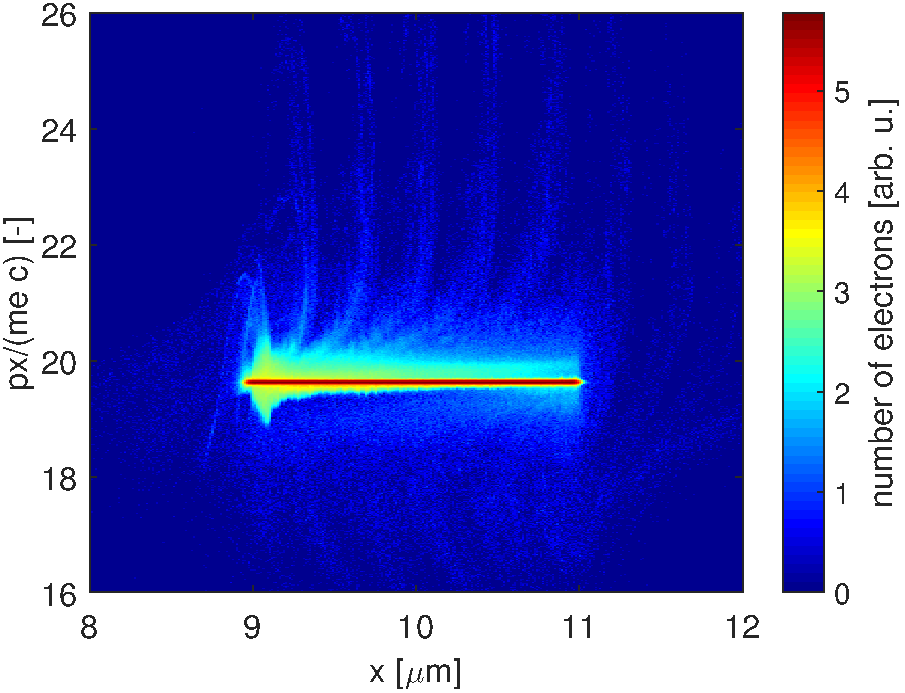
\includegraphics[width=0.45\linewidth]{./img/results/i1e20/05/x_px.pdf}}}
	\sidesubfloat[]{{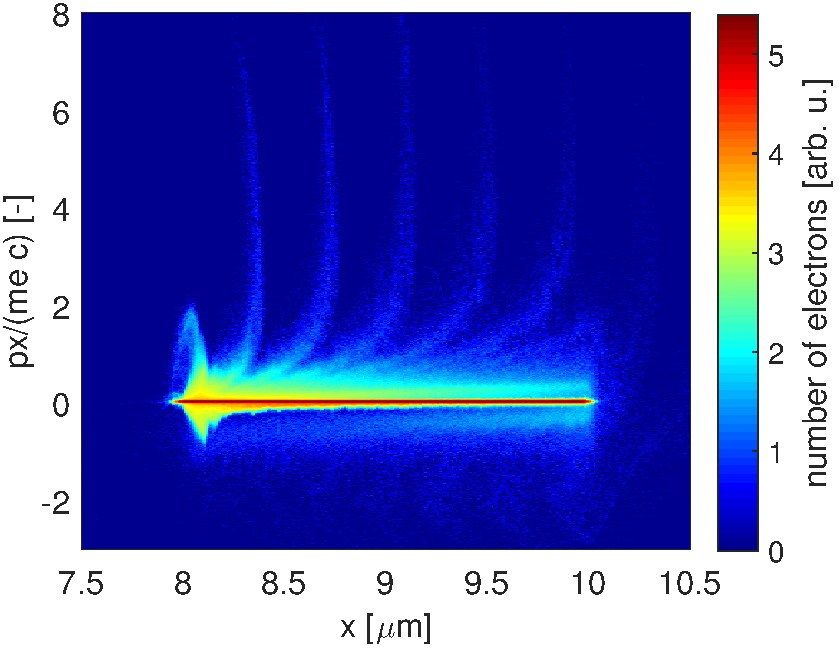
\includegraphics[width=0.45\linewidth]{./img/results/i1e20/2/x_px.pdf}}}\\
	\sidesubfloat[]{{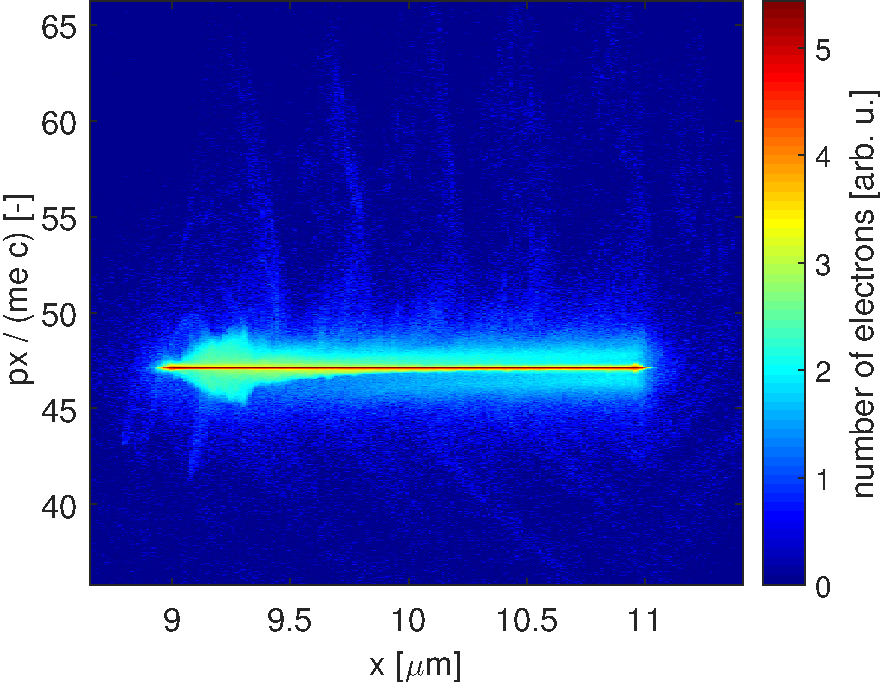
\includegraphics[width=0.45\linewidth]{./img/results/i1e21/05/x_px.pdf}}}
	\sidesubfloat[]{{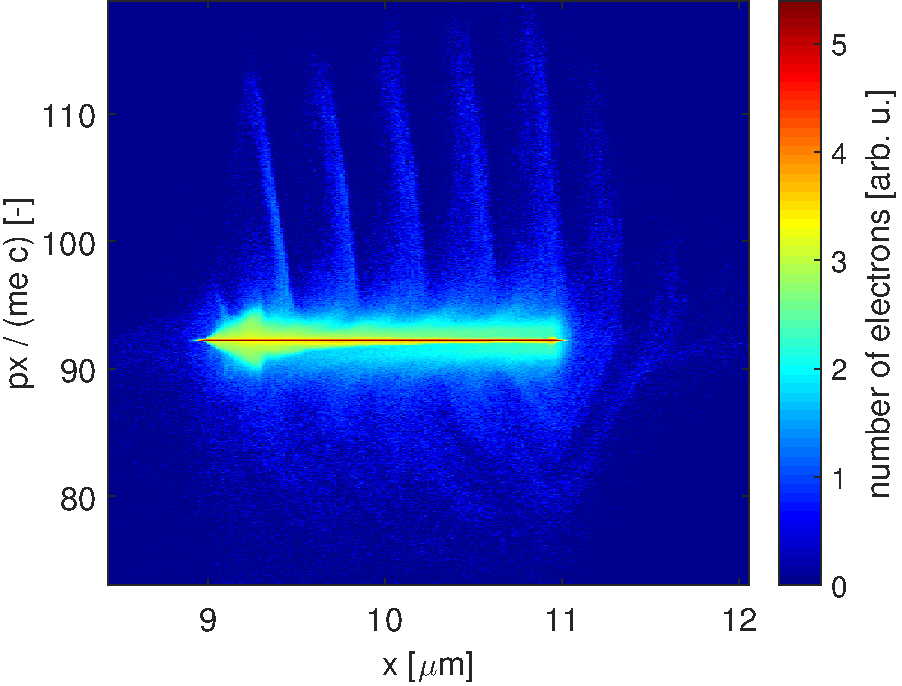
\includegraphics[width=0.45\linewidth]{./img/results/i1e21/2/x_px.pdf}}}
	\caption{\textbf{(a)} w0 = 05 micron, I = 1e20 W/cm2, t = 100 fs \textbf{(b)} w0 = 2 micron, I = 1e20 W/cm2, t = 100 fs \textbf{(c)} w0 = 05 micron, I = 1e21 W/cm2, t = 100 fs \textbf{(d)} w0 = 2 micron, I = 1e21 W/cm2, t = 100 fs}
	\label{}
\end{figure}

\floatsetup[figure]{style=plain, subcapbesideposition=top}
\begin{figure}[h!]
	\centering
	\sidesubfloat[]{{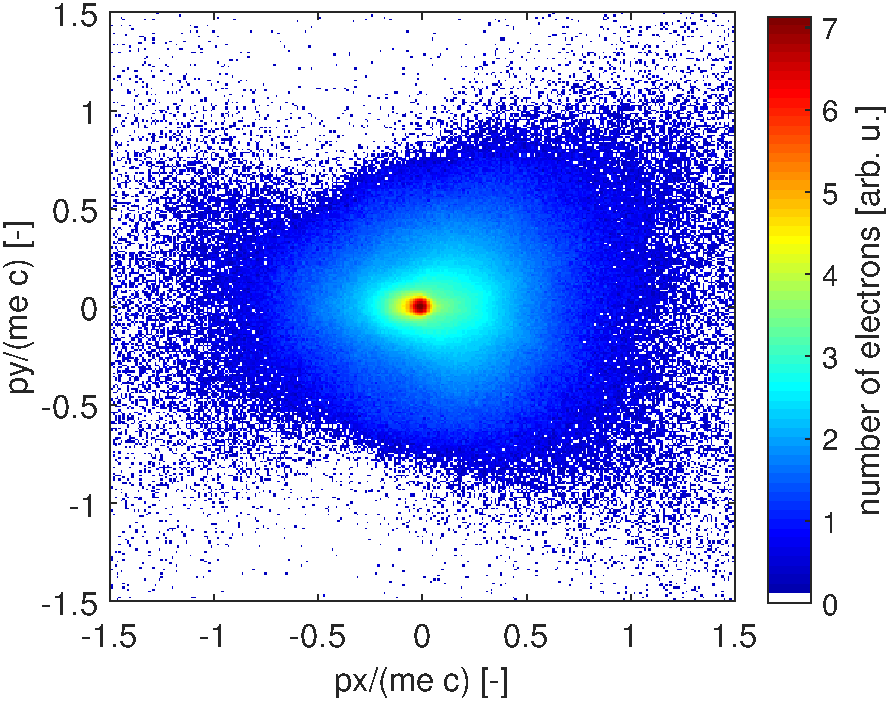
\includegraphics[width=0.45\linewidth]{./img/results/i1e20/05/px_py.pdf}}}
	\sidesubfloat[]{{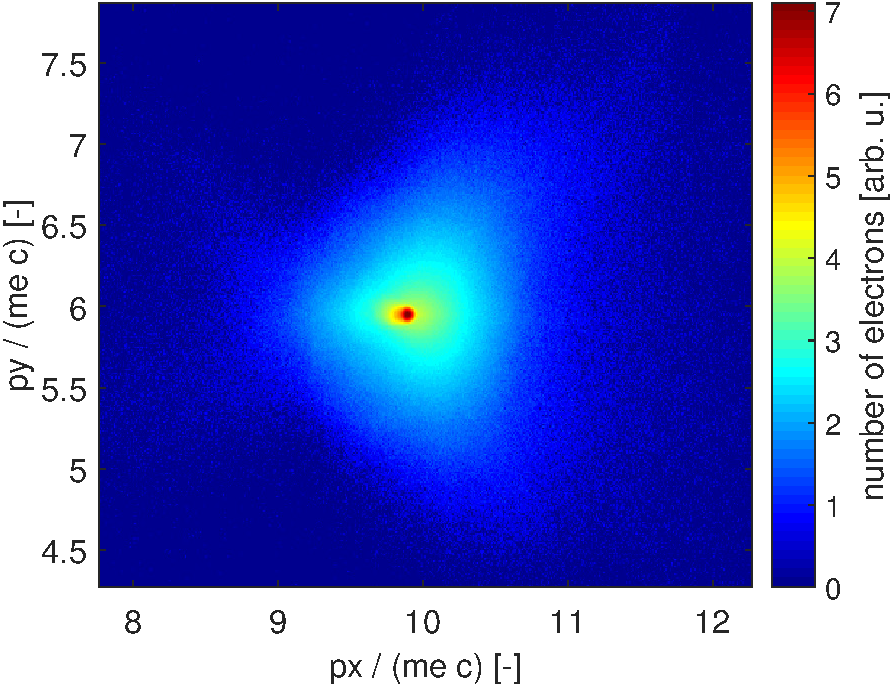
\includegraphics[width=0.45\linewidth]{./img/results/i1e20/2/px_py.pdf}}}\\
	\sidesubfloat[]{{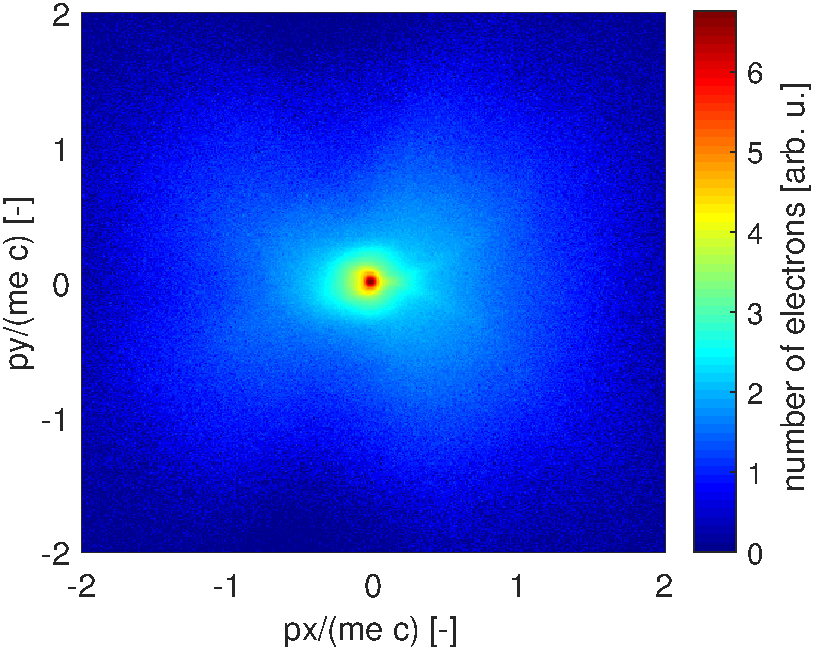
\includegraphics[width=0.45\linewidth]{./img/results/i1e21/05/px_py.pdf}}}
	\sidesubfloat[]{{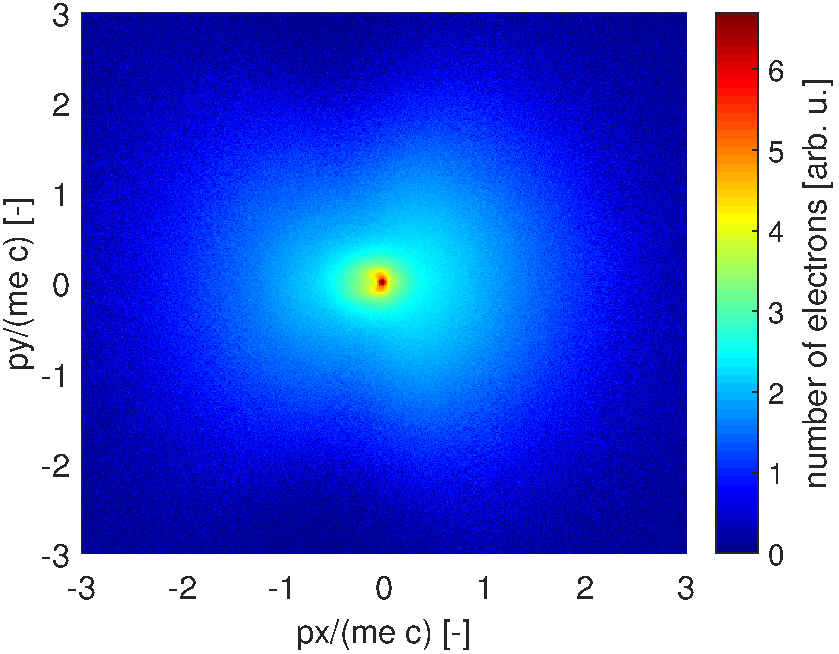
\includegraphics[width=0.45\linewidth]{./img/results/i1e21/2/px_py.pdf}}}
	\caption{\textbf{(a)} w0 = 05 micron, I = 1e20 W/cm2, t = 100 fs \textbf{(b)} w0 = 2 micron, I = 1e20 W/cm2, t = 100 fs \textbf{(c)} w0 = 05 micron, I = 1e21 W/cm2, t = 100 fs \textbf{(d)} w0 = 2 micron, I = 1e21 W/cm2, t = 100 fs}
	\label{}
\end{figure}

\floatsetup[figure]{style=plain, subcapbesideposition=top}
\begin{figure}[h!]
	\centering
	\sidesubfloat[]{{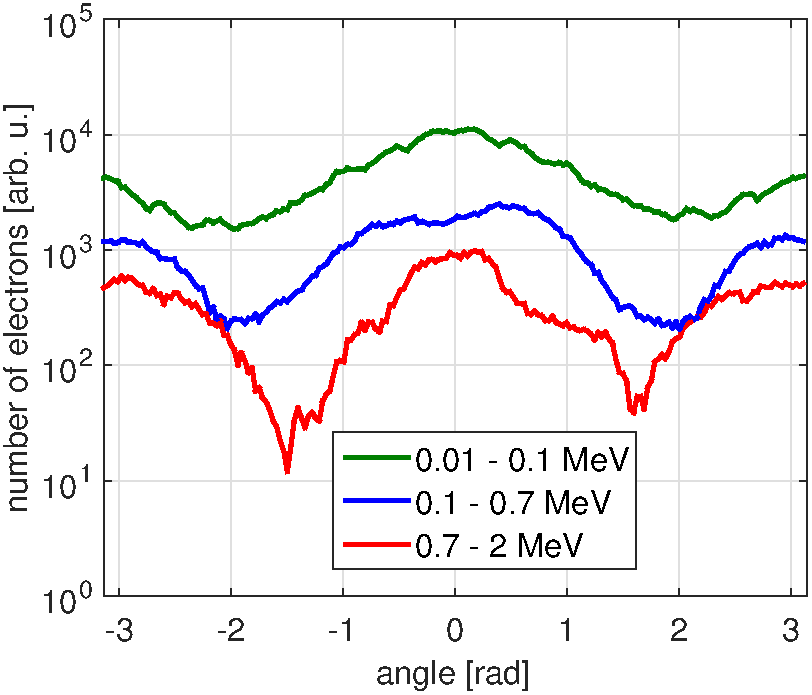
\includegraphics[width=0.45\linewidth]{./img/results/i1e20/05/angles.pdf}}}
	\sidesubfloat[]{{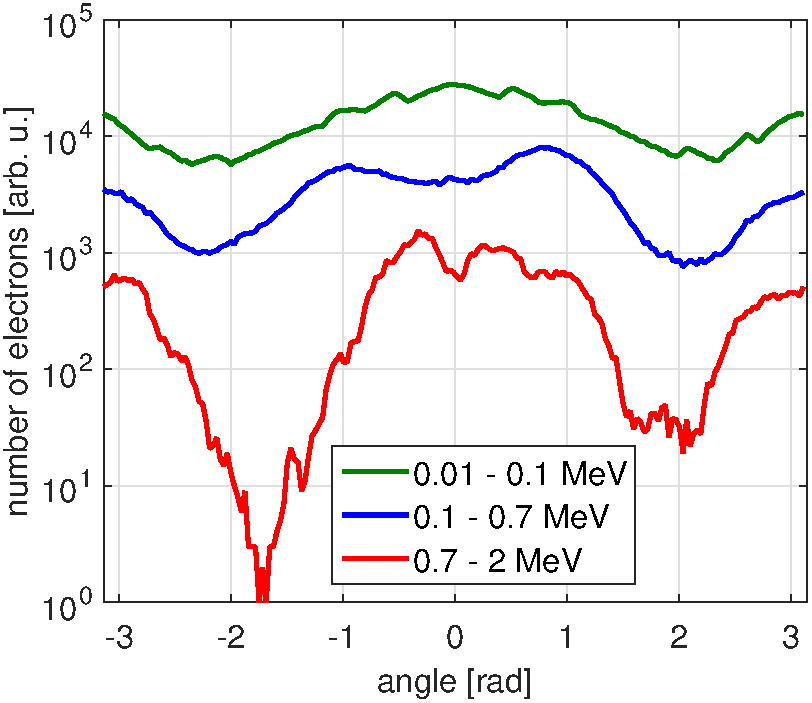
\includegraphics[width=0.45\linewidth]{./img/results/i1e20/2/angles.pdf}}}\\
	\sidesubfloat[]{{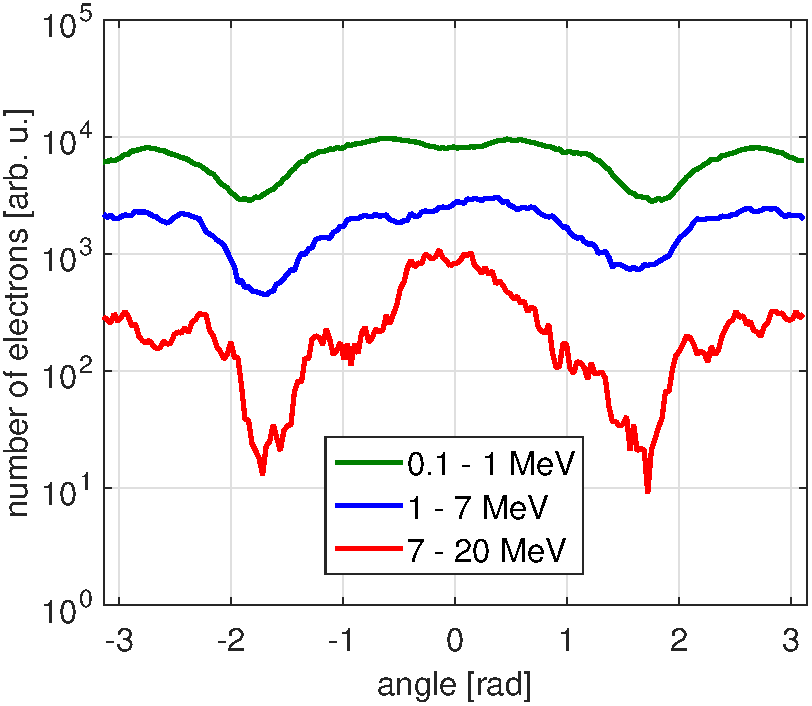
\includegraphics[width=0.45\linewidth]{./img/results/i1e21/05/angles.pdf}}}
	\sidesubfloat[]{{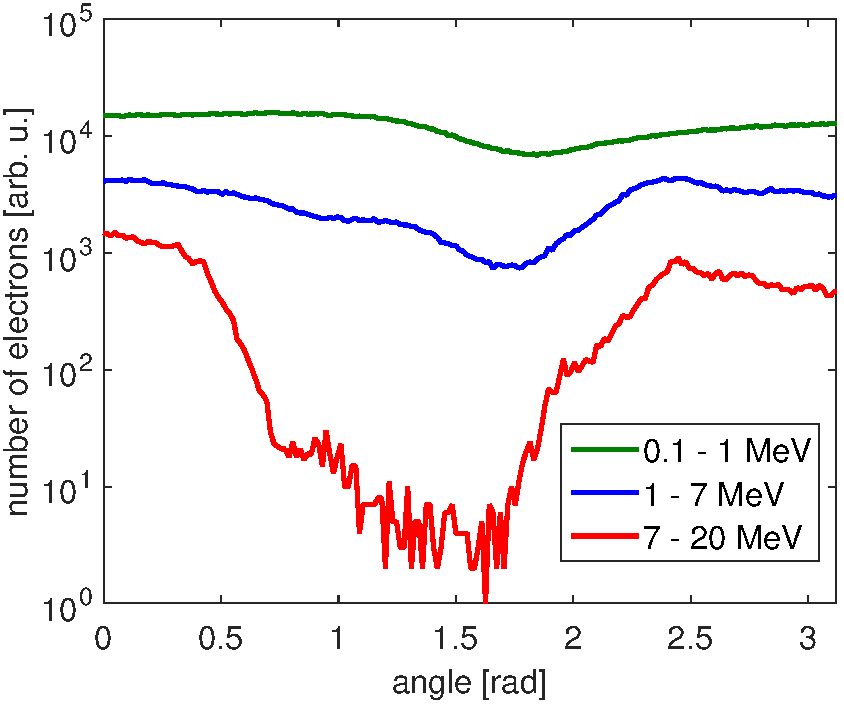
\includegraphics[width=0.45\linewidth]{./img/results/i1e21/2/angles.pdf}}}
	\caption{}
	\label{}
\end{figure}

\floatsetup[figure]{style=plain, subcapbesideposition=top}
\begin{figure}[h!]
	\centering
	\sidesubfloat[]{{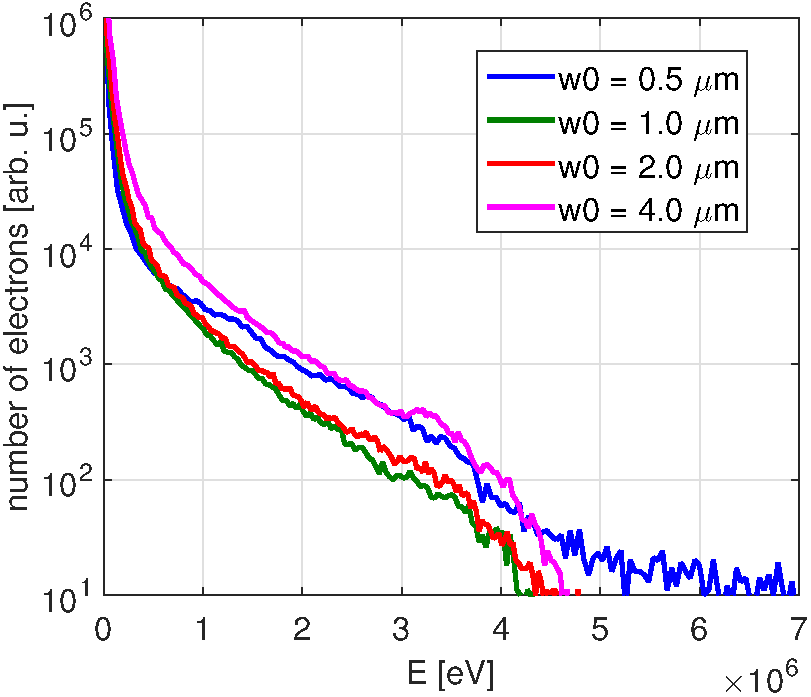
\includegraphics[width=0.45\linewidth]{./img/results/i1e20/dist_e.pdf}}}
	\sidesubfloat[]{{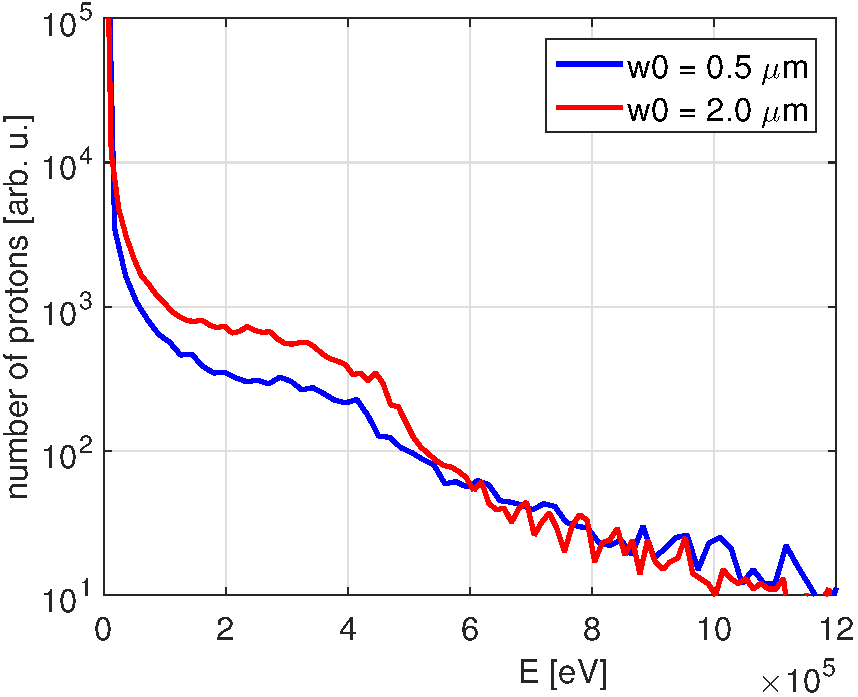
\includegraphics[width=0.45\linewidth]{./img/results/i1e20/dist_p.pdf}}}\\[2mm]
	\sidesubfloat[]{{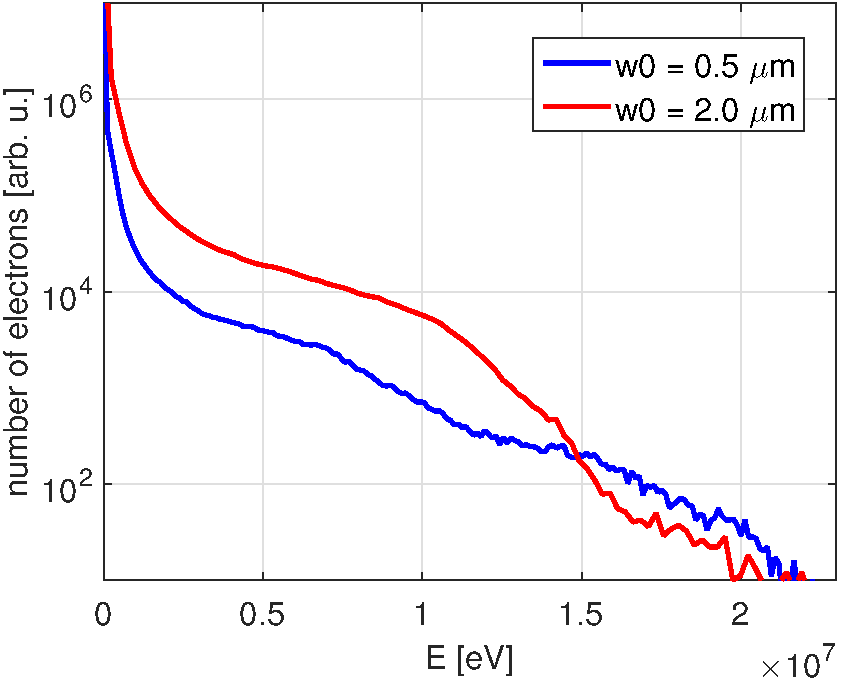
\includegraphics[width=0.45\linewidth]{./img/results/i1e21/dist_e.pdf}}}
	\sidesubfloat[]{{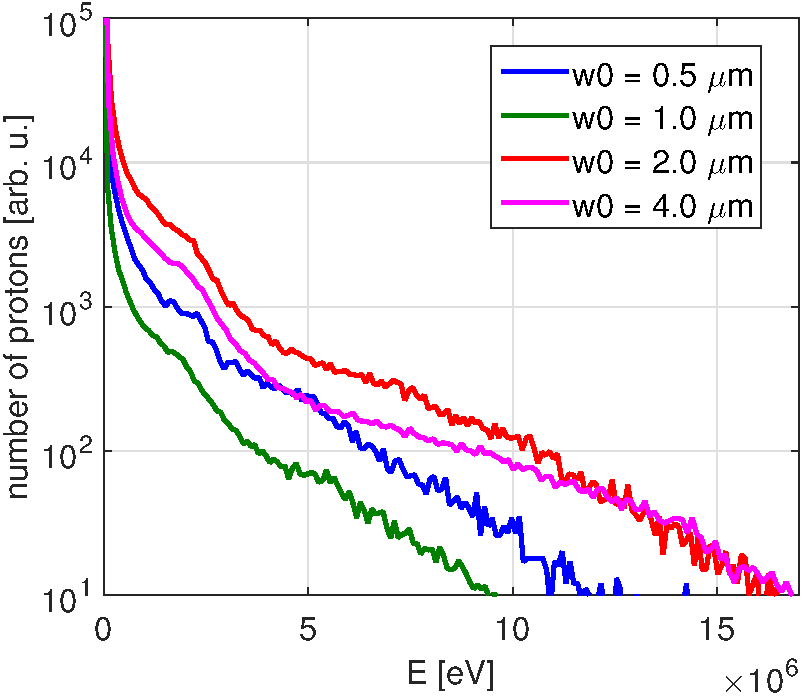
\includegraphics[width=0.45\linewidth]{./img/results/i1e21/dist_p.pdf}}}
	\caption{}
	\label{}
\end{figure}

\floatsetup[figure]{style=plain, subcapbesideposition=top}
\begin{figure}[h!]
	\centering
	\sidesubfloat[]{{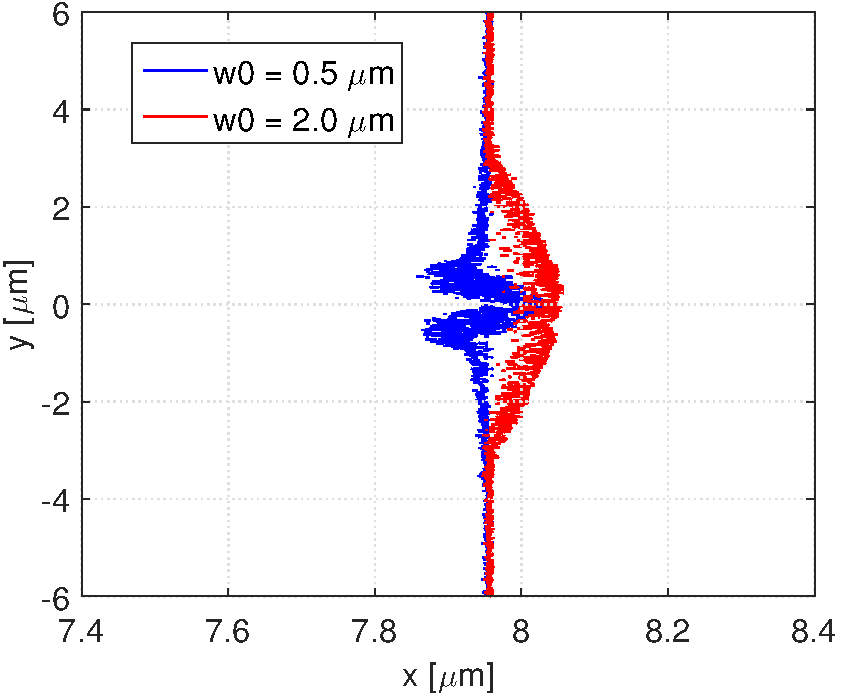
\includegraphics[width=0.445\linewidth]{./img/results/i1e20/dens.pdf}}}
	\hspace{1mm}
	\sidesubfloat[]{{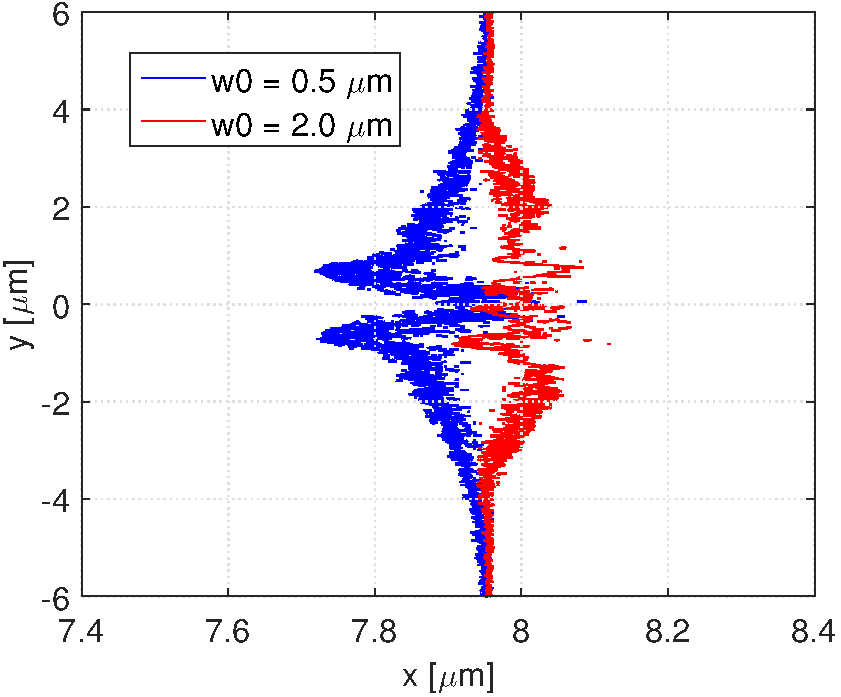
\includegraphics[width=0.445\linewidth]{./img/results/i1e21/dens.pdf}}}
	\caption{\textbf{(a)} nc protons, t = 100 fs, I = 1e20 W/cm2 \textbf{(b)} nc protons, t = 100 fs, I = 1e21 W/cm2}
	\label{}
\end{figure}

\floatsetup[figure]{style=plain, subcapbesideposition=top}
\begin{figure}[h!]
	\centering
	\sidesubfloat[]{{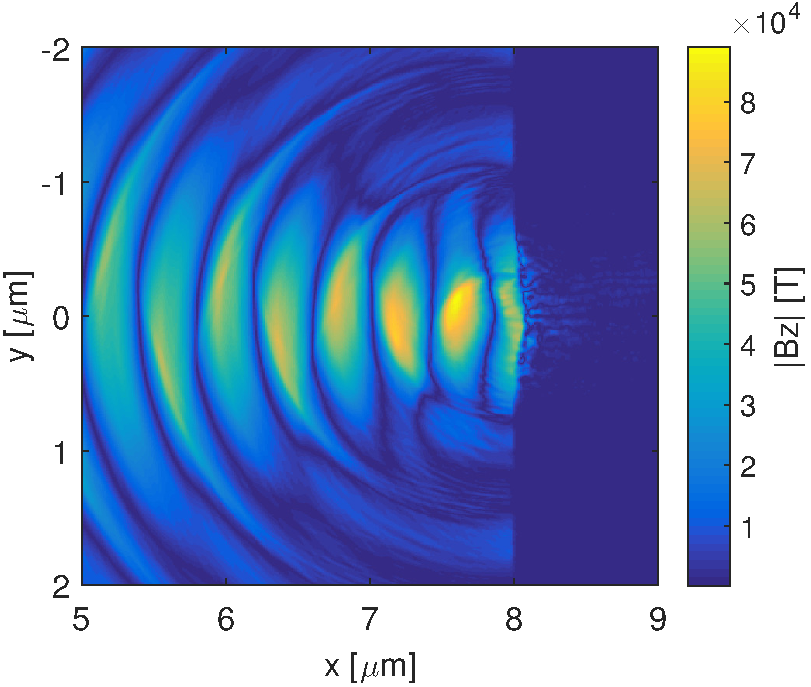
\includegraphics[width=0.45\linewidth]{./img/results/i1e20/05/abs_Bz.pdf}}}
	\sidesubfloat[]{{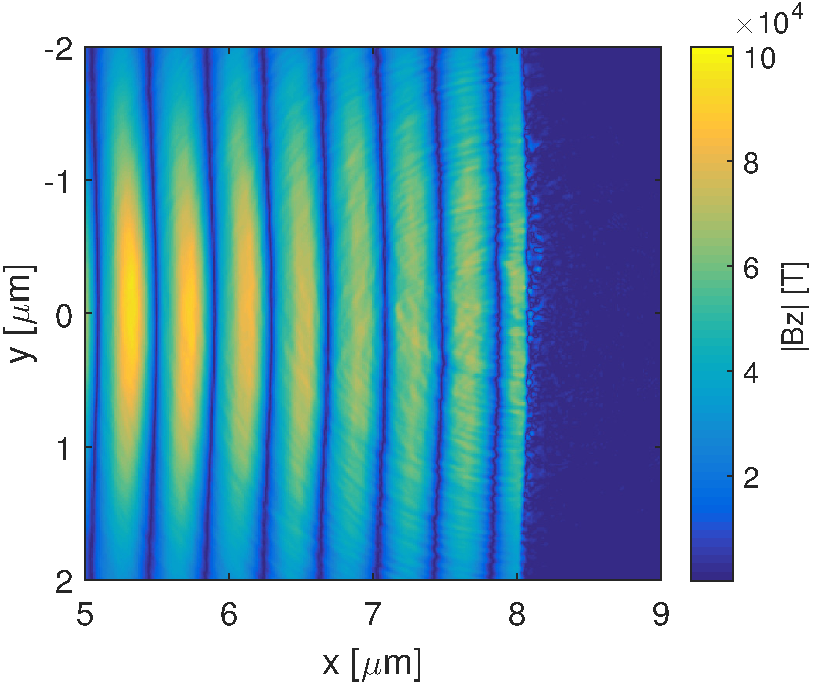
\includegraphics[width=0.45\linewidth]{./img/results/i1e20/2/abs_Bz.pdf}}}\\[2mm]
	\sidesubfloat[]{{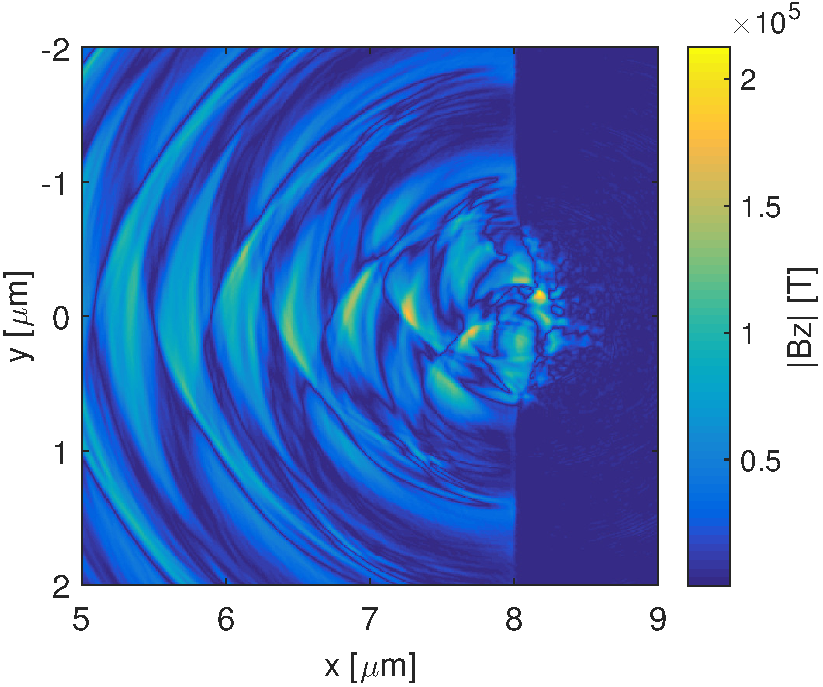
\includegraphics[width=0.45\linewidth]{./img/results/i1e21/05/abs_Bz.pdf}}}
	\sidesubfloat[]{{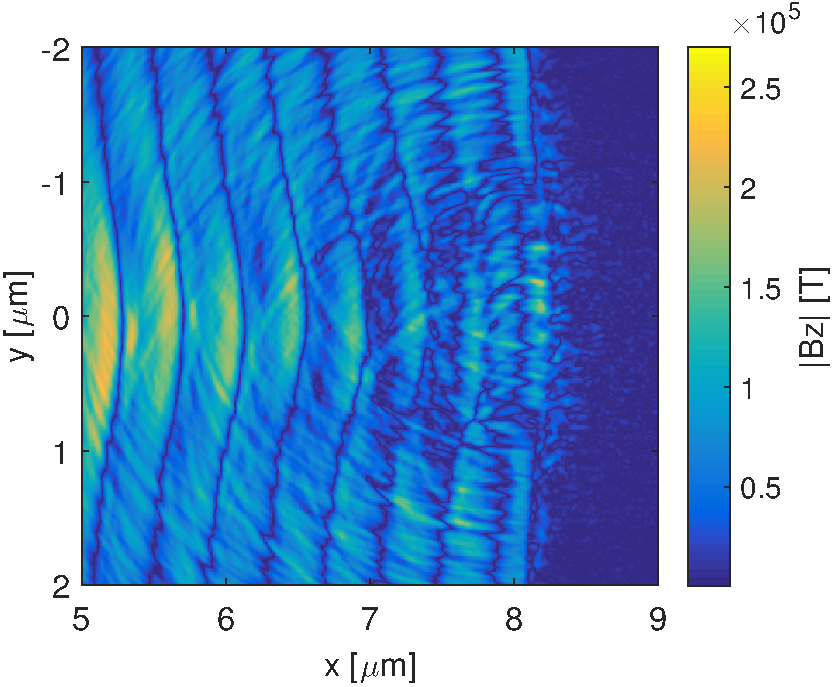
\includegraphics[width=0.45\linewidth]{./img/results/i1e21/2/abs_Bz.pdf}}}
	\caption{}
	\label{}
\end{figure}

\floatsetup[figure]{style=plain, subcapbesideposition=top}
\begin{figure}[h!]
	\centering
	\sidesubfloat[]{{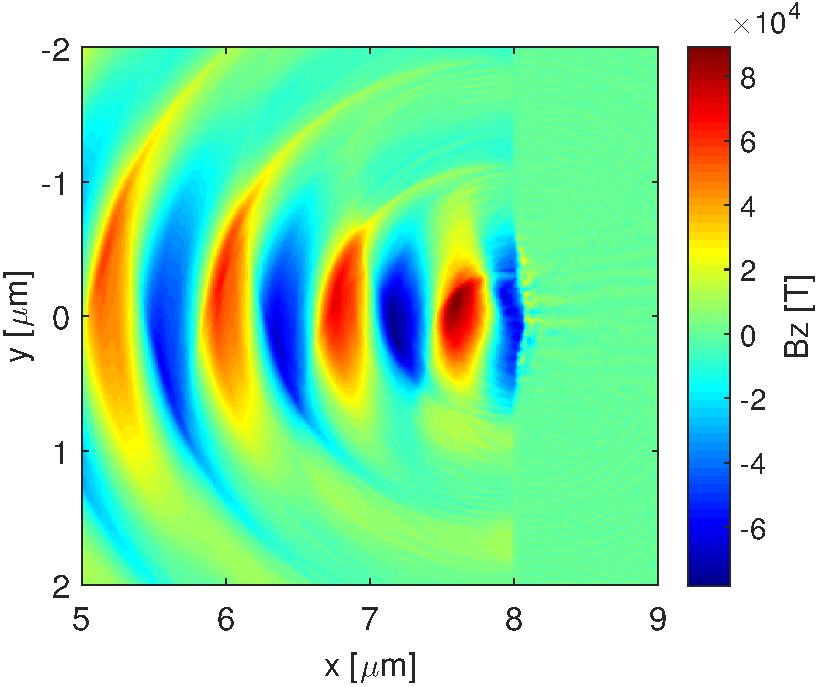
\includegraphics[width=0.45\linewidth]{./img/results/i1e20/05/Bz.pdf}}}
	\sidesubfloat[]{{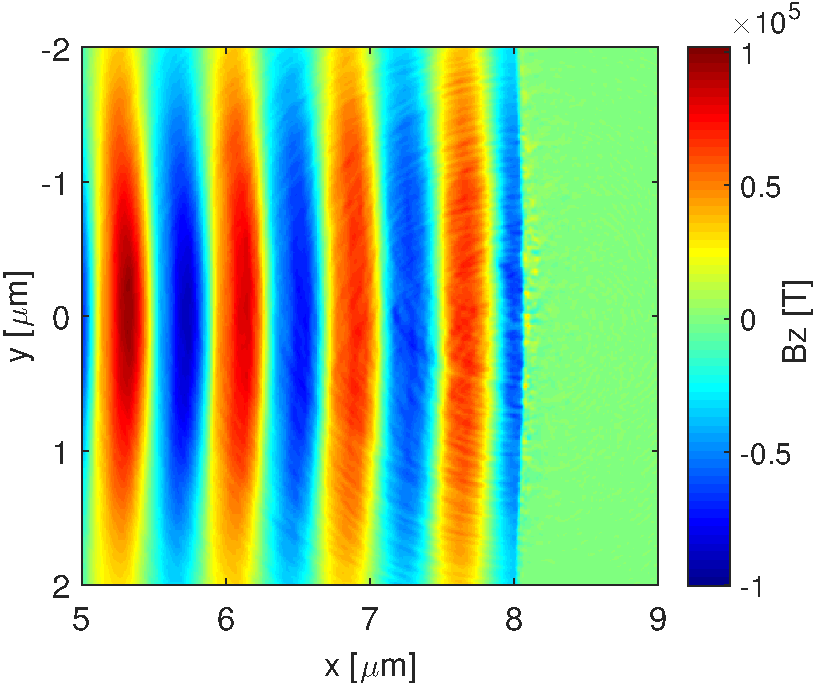
\includegraphics[width=0.45\linewidth]{./img/results/i1e20/2/Bz.pdf}}}\\[2mm]
	\sidesubfloat[]{{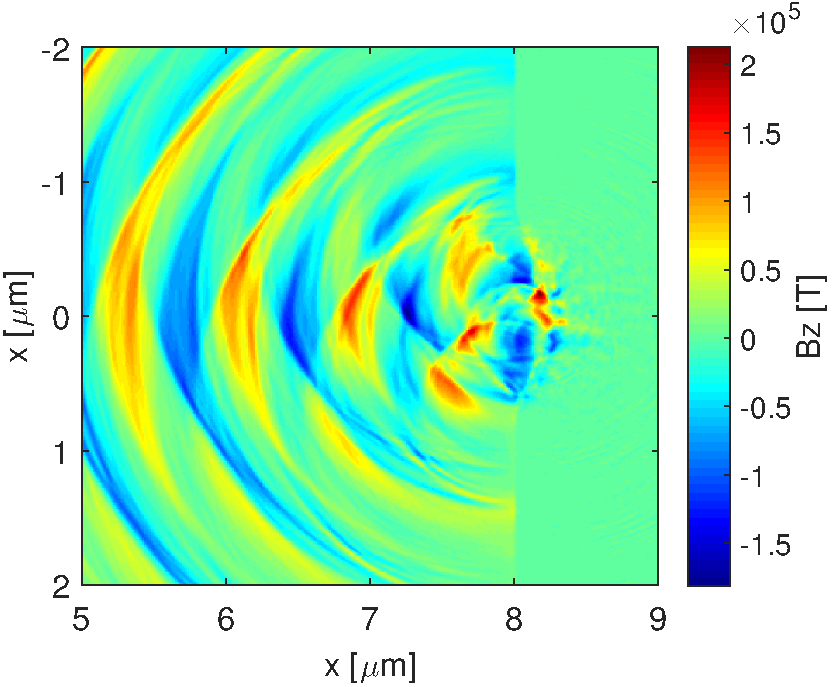
\includegraphics[width=0.45\linewidth]{./img/results/i1e21/05/Bz.pdf}}}
	\sidesubfloat[]{{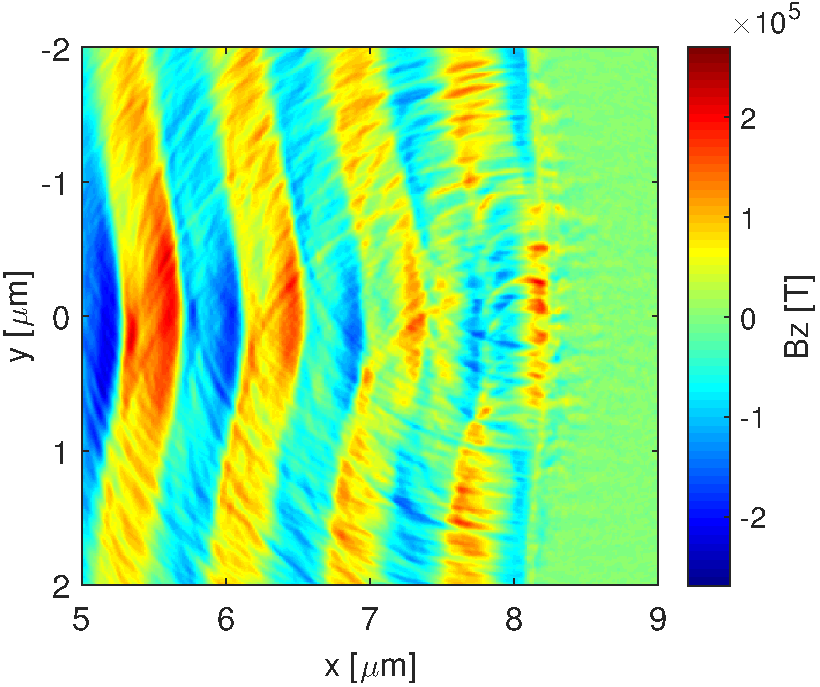
\includegraphics[width=0.45\linewidth]{./img/results/i1e21/2/Bz.pdf}}}
	\caption{}
	\label{}
\end{figure}

\floatsetup[figure]{style=plain, subcapbesideposition=top}
\begin{figure}[h!]
	\centering
	\sidesubfloat[]{{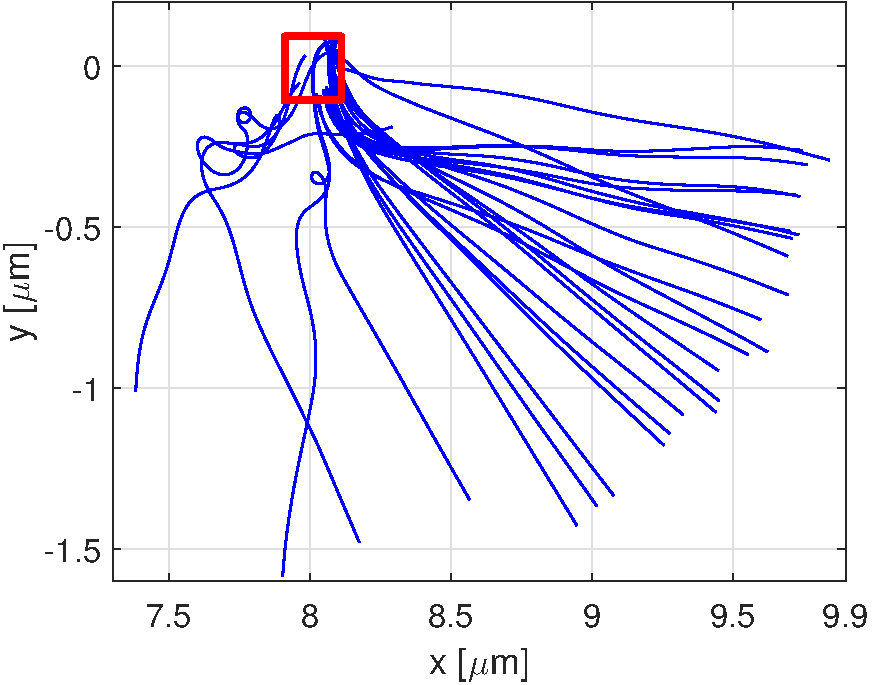
\includegraphics[width=0.445\linewidth]{./img/results/i1e21/05/trajectories.pdf}}}
	\hspace{1mm}
	\sidesubfloat[]{{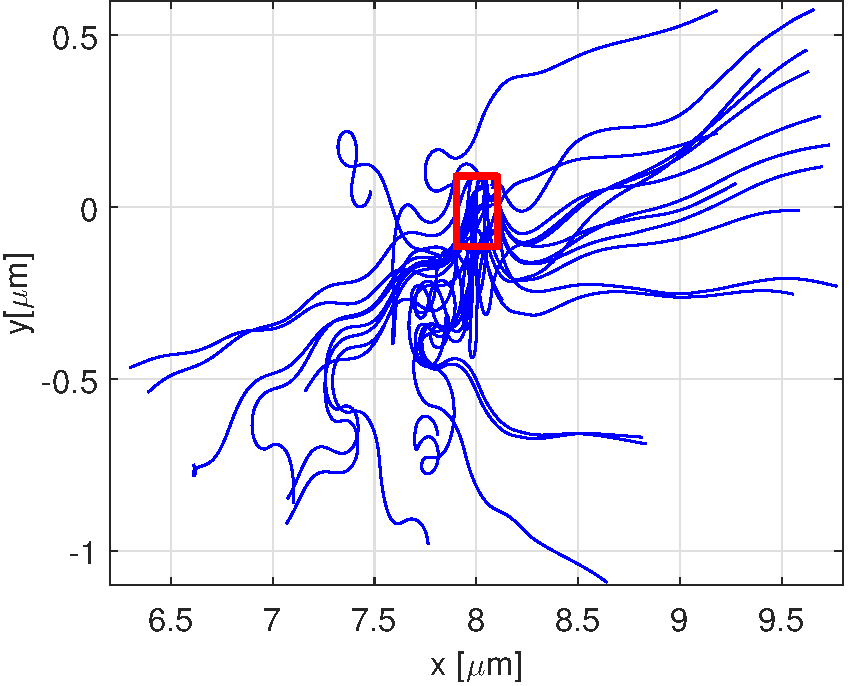
\includegraphics[width=0.445\linewidth]{./img/results/i1e21/2/trajectories.pdf}}}
	\caption{\textbf{(a)} electrons, w0 = 0.5 micron, t = 100 fs, I = 1e21 W/cm2 \textbf{(b)} electrons, wo = 2 micron, t = 100 fs, I = 1e21 W/cm2}
	\label{}
\end{figure}

\floatsetup[figure]{style=plain, subcapbesideposition=top}
\begin{figure}[h!]
	\centering
	\sidesubfloat[]{{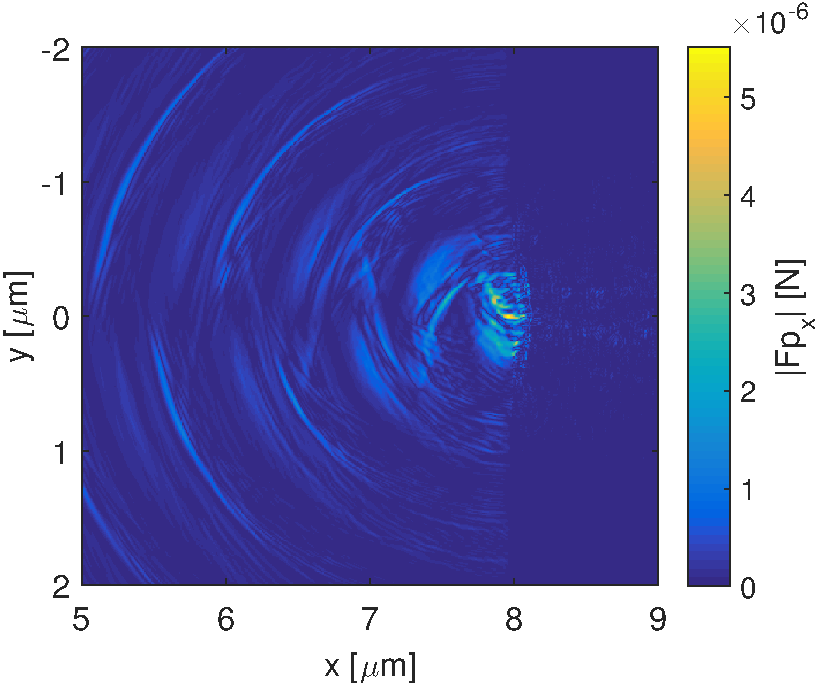
\includegraphics[width=0.45\linewidth]{./img/results/i1e20/05/abs_Fpx.pdf}}}
	\sidesubfloat[]{{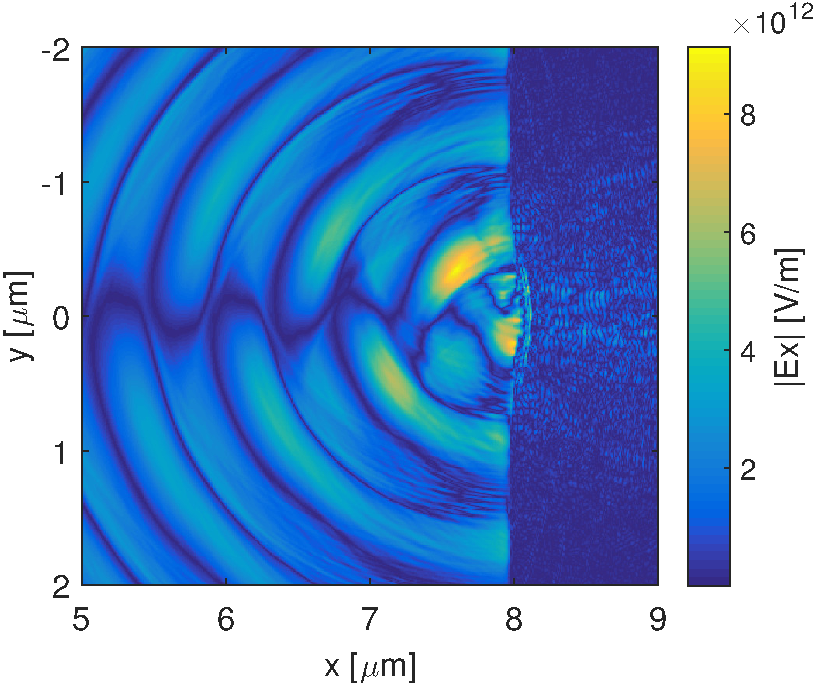
\includegraphics[width=0.45\linewidth]{./img/results/i1e20/05/abs_Ex.pdf}}}\\
	\sidesubfloat[]{{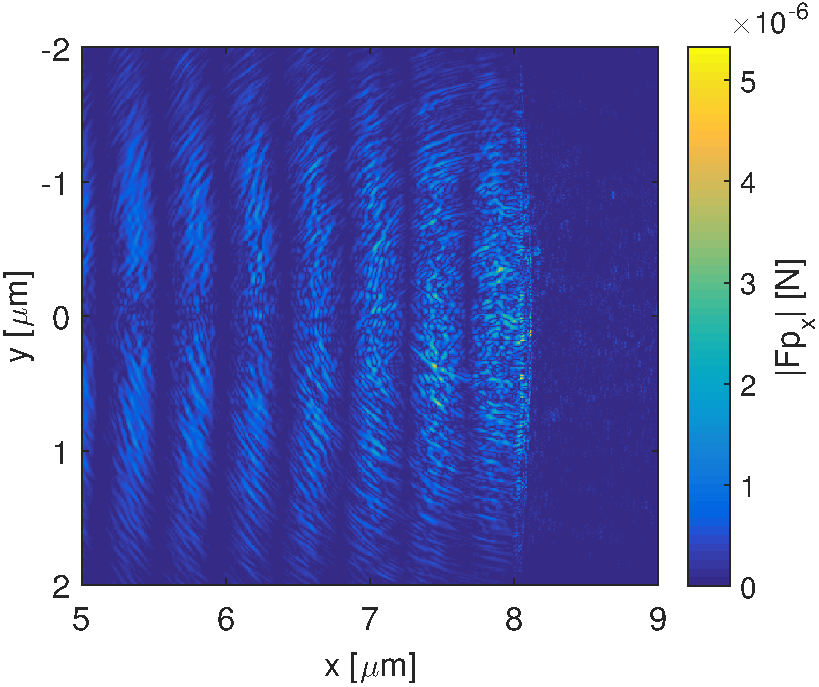
\includegraphics[width=0.45\linewidth]{./img/results/i1e20/2/abs_Fpx.pdf}}}
	\sidesubfloat[]{{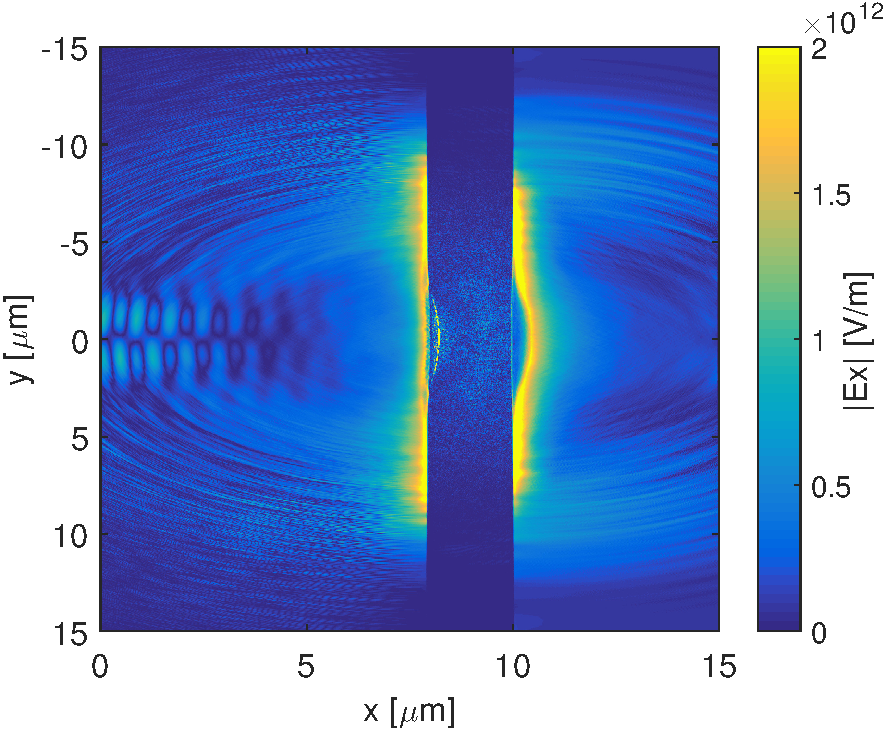
\includegraphics[width=0.45\linewidth]{./img/results/i1e20/2/abs_Ex.pdf}}}
	\caption{}
	\label{}
\end{figure}

\floatsetup[figure]{style=plain, subcapbesideposition=top}
\begin{figure}[h!]
	\centering
	\sidesubfloat[]{{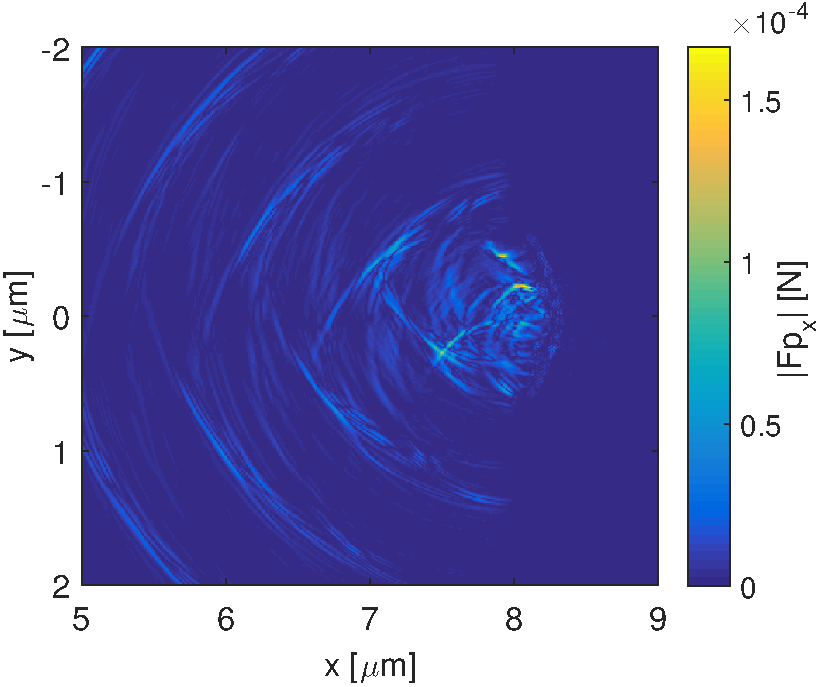
\includegraphics[width=0.45\linewidth]{./img/results/i1e21/05/abs_Fpx.pdf}}}
	\sidesubfloat[]{{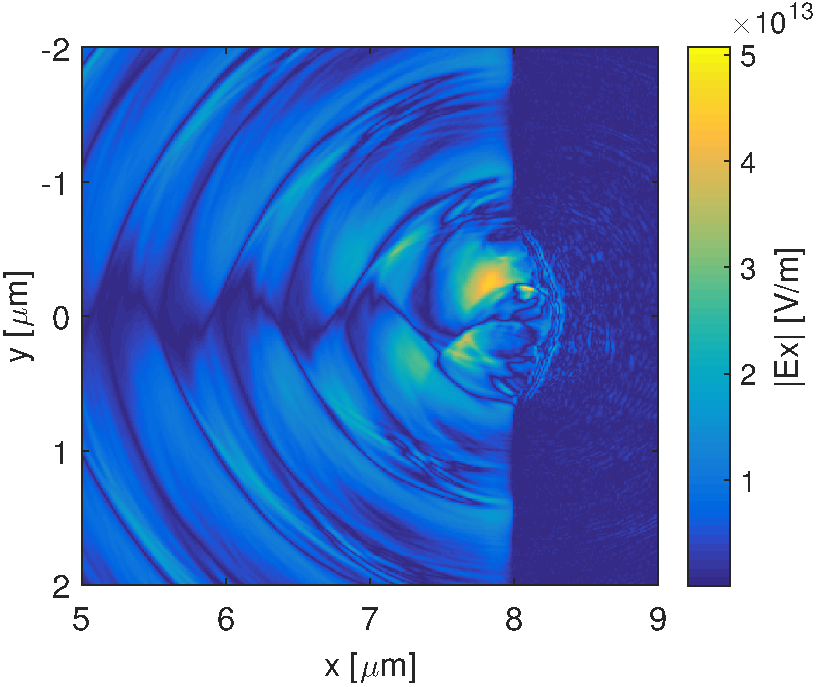
\includegraphics[width=0.45\linewidth]{./img/results/i1e21/05/abs_Ex.pdf}}}\\
	\sidesubfloat[]{{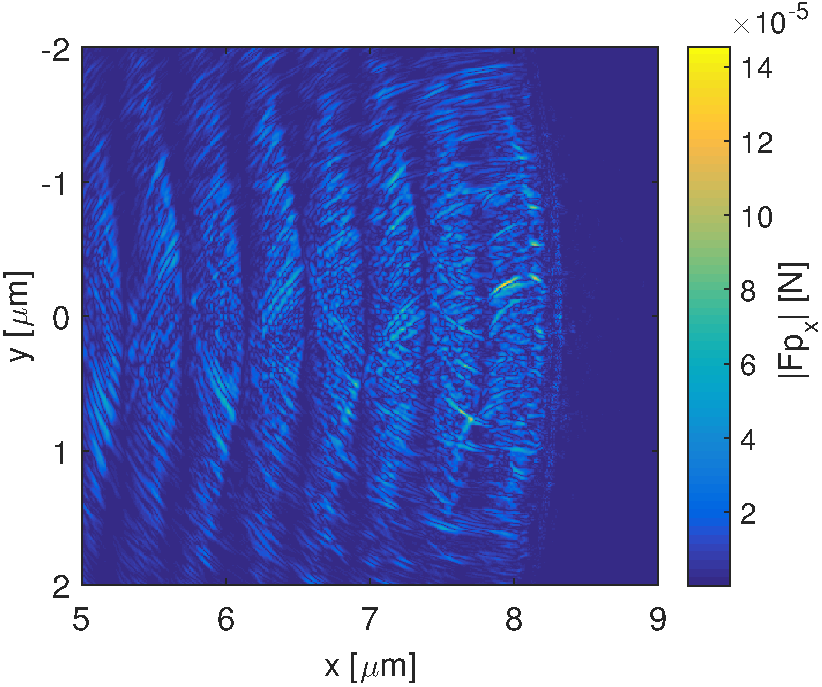
\includegraphics[width=0.45\linewidth]{./img/results/i1e21/2/abs_Fpx.pdf}}}
	\sidesubfloat[]{{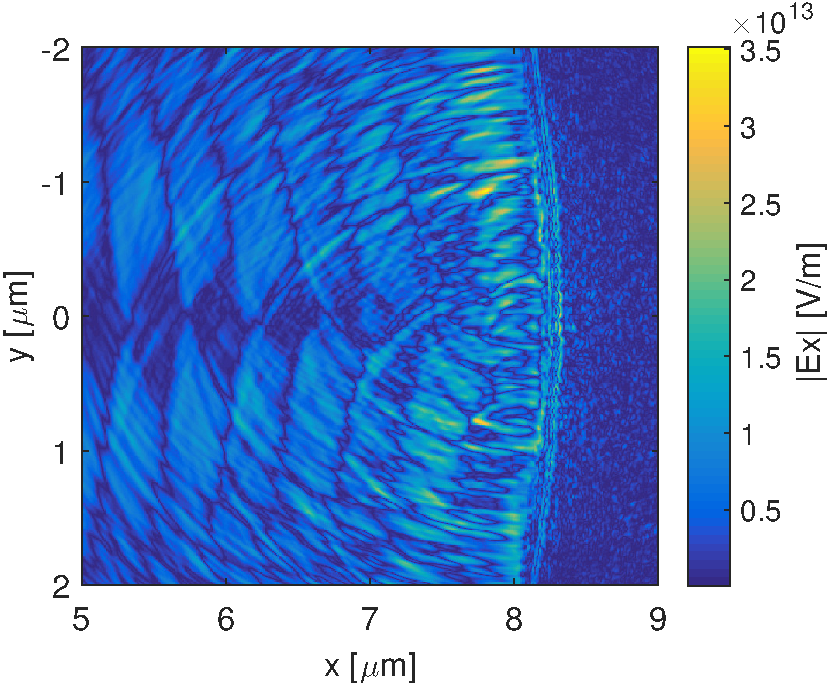
\includegraphics[width=0.45\linewidth]{./img/results/i1e21/2/abs_Ex.pdf}}}
	\caption{}
	\label{}
\end{figure}